\chapter{Tools from Differential Geometry}\label{ch:tools}

\begin{flushright}
\emph{Give me six hours to chop down a tree\\ and I will spend the first four sharpening the axe.}
\\ -Abraham Lincoln
\end{flushright}

\vspace{0.6cm}

% % % % % % % % % % % % % % % % % % % % % % % % % % % % % % % % % % % % % %
% % % % % % % % % % % % % % % % % % % % % % % % % % % % % % % % % % % % % %
% % 
% % % % % % % % % % % % % % % % % % % % % % % % % % % % % % % % % % % % % %
% % % % % % % % % % % % % % % % % % % % % % % % % % % % % % % % % % % % % %
\section{A Lie Group Structure for the Set of Transformations}\label{se:finite_lie_group}

%%introductory definition
We consider every group $\mathbb{G}$ as a group of transformations acting on $\mathbb{R}^{d}$, having in mind the particular case $d=2,3$ for 2-dimensional or 3-dimensional images.
We will focus our attention to transformations defined by matrices or diffeomorphism. Other than group they also have the structure of Lie group: they are considered with a maximal atlas that makes them differentiable manifold, in which the composition of two transformations and the inverse of each transformation are well defined differentiable maps:
\begin{align*}
\mathbb{G} \times \mathbb{G} & \longrightarrow  \mathbb{G}    \\
(x,y) &\longmapsto  x y^{-1}
\end{align*}

Differential geometry is, generally speaking, a technique to use the well known calculus features and operators on spaces different from the usual $\mathbb{R}^{n}$. Adding the differentiable structure to a group of transformations provides new handles to hold and manipulate them; in particular it provides the opportunity to define a tangent space to each point of the group (and so a fiber bundle), a space of vector fields, a set of flows and one parameter subgroup as well as other features that enrich this structure.

Due to space limitations we will refer to \cite{do1976differential} and \cite{lee2012introduction} for the definitions and concepts of differential geometry and \cite{do1992riemannian} for definition and concepts of Riemannian geometry.

% % % % % % % % % % % % % % % % % % % % % % % % % % % % % % % % % % % % % %
% % SECTION
% % % % % % % % % % % % % % % % % % % % % % % % % % % % % % % % % % % % % % 
\section{Lie Exponential, Lie logarithm, Lie log-composition and the BCH formula}\label{se:lie_exp_log_comp_bch}
Let $\mathbf{v}$ be an element in the tangent space $\mathfrak{g}$ of the Lie group $\mathbb{G}$.
The \emph{Lie exponential} is defined as 
\begin{align*}
\exp :  \mathfrak{g} & \longrightarrow  \mathbb{G}  \\
\mathbf{v} &\longmapsto  \exp(\mathbf{v} ) = \gamma(1) %\quad \dot{\gamma}(t) = V_{\gamma(t)}, \gamma(0) = e
\end{align*}
where $\gamma: [0,1]\rightarrow \mathbb{G} $ is the unique one-parameter subgroup of $\mathbb{G}$ having $\mathbf{v}$ as its tangent vector at the identity. The identity is indicated with $e$ for the general case, $I$ for matrices and $1$ for diffeomorphisms.
The exponential map satisfies the following properties:
\begin{enumerate}
	\item $\exp(t\mathbf{v}) =\gamma(t) $.
	\item $\exp(\mathbf{v}) = e$ if $\mathbf{v} = \mathbf{0}$.
	\item $\exp(\mathbf{v})\circ \exp(\mathbf{-v})  = e$
	\item As a direct consequence of the definition here provided, based on the one parameter subgroup, it follows that:
	\begin{align*}
	\exp((t+s)\mathbf{v}) = \gamma(t+s) = \gamma(t)\circ \gamma(s) = \exp(t\mathbf{v})\exp(s\mathbf{v})
	\end{align*}
	This in particular is one of the reasons that justifies the name exponential for a maps between structures in differential geometry.
	\item $\exp(\mathbf{v})$ is invertible and $(\exp(\mathbf{v}))^{-1} = \exp(-\mathbf{v})$.
		\item  $\exp(\mathbf{u} + \mathbf{v}) =\lim_{m\rightarrow \infty} (\exp(\frac{\mathbf{v}}{m}) \circ\exp(\frac{\mathbf{v}}{m}))^{m}$
	\item $\exp$ is a local isomorphism: it is an isomorphisms between a neighborhood of $\mathbf{0}$ in $\mathfrak{g}$ to a neighborhood of $e$ in $\mathbb{G}$.
	\item If $\exp(\mathbf{w}) = \exp(\mathbf{u})  \exp(\mathbf{v})$ then 
	\begin{align}\label{prop:lie_inversion_property}
	\exp(\mathbf{-w}) = \exp(\mathbf{-v}) \exp(\mathbf{-u})
	\end{align}
\end{enumerate}
\begin{proof}
	We will present only the last statement leaving the others to the literature. The hypothesis $\exp(\mathbf{w}) = \exp(\mathbf{v}) \circ \exp(\mathbf{u})$ follows the subsequent chain of implications (each algebraic passage involves a geometrical construction, not shown here for brevity):
	\begin{align*}
		\exp(\mathbf{w}) &= \exp(\mathbf{v}) \circ \exp(\mathbf{u}) \\
		\exp(-\mathbf{w}) \circ \exp(\mathbf{w}) &= \exp(-\mathbf{w}) \circ\exp(\mathbf{v}) \circ \exp(\mathbf{u}) \\
		e &= \exp(-\mathbf{w}) \circ\exp(\mathbf{v}) \circ \exp(\mathbf{u}) \\
		\exp(-\mathbf{u})  &= \exp(-\mathbf{w}) \circ\exp(\mathbf{v})  \\
		\exp(-\mathbf{u}) \circ\exp(-\mathbf{v})  &= \exp(-\mathbf{w})  
	\end{align*}
\end{proof}
The neighborhoods of $\mathbb{G}$ and of $\mathfrak{g}$ such that the last property holds, are called \emph{internal cut locus} of $\mathbb{G}$ and $\mathfrak{g}$ respectively. The \emph{cut locus} is the boundary of the internal cut locus.

When we deal with a matrix Lie group of dimension $n$, the composition in the Lie group consists in the matrix product and we have the following remarkable properties \cite{hall2015lie}, \cite{kirillov2008introduction}:
\begin{enumerate}
	\item for all $\mathbf{v}$ in a matrix Lie algebra $\mathfrak{g}$:
	\begin{align}\label{eq:exp_as_inf_sum}
	\exp(\mathbf{v}) = \sum_{k=0}^{\infty} \frac{\mathbf{v}^{k}}{k!}
	\end{align}
	\item If $\mathbf{u}$ and $\mathbf{v}$ are commutative then $\exp(\mathbf{u} + \mathbf{v}) = \exp(\mathbf{u})\exp(\mathbf{v})$.
	\item If $\mathbf{c}$ is an invertible matrix then $\exp(\mathbf{c}\mathbf{v}\mathbf{c}^{-1}) = \mathbf{c}\exp(\mathbf{v})\mathbf{c}^{-1}$.
	\item $\det(\exp(\mathbf{v})) = \exp(\text{trace}(\mathbf{v}))$
	\item For any norm, $\euclideanMetric{\exp(\mathbf{v})} \leq \exp(\euclideanMetric{\mathbf{v}})$.
\end{enumerate}

The idea of defining an inverse of the Lie exponential leads to the idea of the Lie logarithm, defined as
\begin{align*}
\log : \mathbb{G} & \longrightarrow \mathfrak{g} \\
\varphi &\longmapsto \log (\varphi)  =  \mathbf{v}   
\end{align*}
where $\mathbf{v}$ is the tangent vector having $\varphi$ as it $\exp$.

\noindent
If $\mathbb{G}$ is a matrix Lie group of dimension $n$, the following properties hold:
\begin{enumerate}
	\item for all $\varphi$ in the matrix Lie group $\mathbb{G}$:
	\begin{align}\label{eq:log_as_inf_sum}
	\log(\mathbf{\varphi}) = \sum_{k=1}^{\infty}(-1)^{k+1} \frac{(\varphi-I)^{k} }{k}
	\end{align}
	Having indicated the identity matrix with $I$.
	\item For any norm, and for any $n\times n$ matrix $\mathbf{c}$, exists an $\alpha$ such that 
	\begin{align}\label{eq:prop_matrix_diff_log}
	\euclideanMetric{ \log(I + \mathbf{c}) - \mathbf{c} }  \leq \alpha \euclideanMetric{ \mathbf{c}}^{2}
	\end{align}
	\item For any $n\times n$ matrix $\mathbf{c}$ and for any sequence of matrix $\{\mathbf{d}_{j}\}$ such that  $\euclideanMetric{ \mathbf{d}_{j}} \leq \alpha/j^2$ it follows:
	\begin{align}\label{eq:prop_matrix_lim}
	\lim_{k\rightarrow \infty} \big( I + \frac{\mathbf{c}}{k} + \mathbf{d}_{k} \big)^{k} = \exp{(\mathbf{c})}
	\end{align}
\end{enumerate} 

The \emph{Lie log-composition} (because based on the Lie logarithm and Lie exponential maps) is defined here as the inner binary operation on the Lie algebra that reflects the composition on the lie group:
\begin{align*}
\oplus : \mathfrak{g} \times \mathfrak{g} & \longrightarrow \mathfrak{g}    \\
(\mathbf{v}_{1}, \mathbf{v}_{2}) &\longmapsto \mathbf{v}_{1}\oplus \mathbf{v}_{2} =  \log(\exp(\mathbf{v}_1)\circ \exp(\mathbf{v}_2))
\end{align*}

\noindent
The following properties holds for the Lie log-composition:
\begin{enumerate}
	\item $\mathfrak{g} $ with the Lie log-composition $\oplus$ is a local topological non-commutative group (local group for short): if $C_{\mathfrak{g}}$ is the internal cut locus of $\mathfrak{g}$ then:
	\begin{enumerate}
		\item $(\mathbf{u}_{1}\oplus\mathbf{u}_{2}) \oplus \mathbf{u}_{3}
		= \mathbf{u}_{1}\oplus(\mathbf{u}_{2} \oplus \mathbf{u}_{3})$ for all $\mathbf{u}_{1}, \mathbf{u}_{2}, \mathbf{u}_{3}$ in $C_{\mathfrak{g}}$.
		\item $\mathbf{u}\oplus\mathbf{0}  = \mathbf{0}\oplus\mathbf{u} = \mathbf{u}$ for all $\mathbf{u}$ in $C_{\mathfrak{g}}$.
		\item $\mathbf{u}\oplus(-\mathbf{u} ) = \mathbf{0}$ for all $\mathbf{u}$ in $C_{\mathfrak{g}}$.
	\end{enumerate}
	\item For all $t,s$ real, such that $(t+s)\mathbf{u}$ is in $C_{\mathfrak{g}}$,
	\begin{align*}
	(t\mathbf{u})\oplus (s\mathbf{u}) = (t+s)\mathbf{u}
	\end{align*}
	And in particular, if the Lie algebra $\mathfrak{g}$ has dimension $1$ the local group structure is compatible with the additive group of the vector space $\mathfrak{g}$.
\end{enumerate}

\noindent
The algebraic structure $(\mathfrak{g} , \oplus)$ is called Lie log-group. Additional observations on this algebraic structure in the particular case of diffeomorphisms, are proposed in the next chapter.

To compute the log-composition there is the Backer-Campbell-Hausdorff formula, or BCH,
that provides the exact solution to the log-composition: 
\begin{align*}
BCH(\mathbf{u},\mathbf{v}) 
= 
\mathbf{u} + \mathbf{v} + \frac{1}{2}[\mathbf{u},\mathbf{v}] + \frac{1}{12}([\mathbf{u},[\mathbf{u},\mathbf{v}]]
+ [\mathbf{v},[\mathbf{v},\mathbf{u}]]) - \frac{1}{24}[\mathbf{v},[\mathbf{u},[\mathbf{u},\mathbf{v}]]] +... 
\end{align*}
Ironically, the name of the formula does not refer to Dynkin, who originally developed the proof of the equality in 1947 \cite{dynkin1947calculation}. An nice introduction to the particular case of matrices can be found in \cite{hall2015lie}; while the general case is presented in \cite{klarsfeld1989baker}, \cite{serre2009lie}, and for application to medical imaging \cite{lorenzi2014efficient}, \cite{vercauteren08}.
This expansion provides the most immediate way to obtain a numerical computation of $\mathbf{u}\oplus \mathbf{v}$, by truncating its terms, but as stated in the introduction, chapter \ref{ch:introduction} this approximation can be problematic.

% % % % % % % % % % % % % % % % % % % % % % % % % % % % % % % % % % % % % %
% % 
% % % % % % % % % % % % % % % % % % % % % % % % % % % % % % % % % % % % % % 
\section{Affine Exponential Affine Logarithm and Parallel Transport: Definitions and Properties}\label{se:pt}

Considering a Lie Group $\mathbb{G}$ with a connection $\nabla$, the vector field $\nabla_{U}(V)$ associates at each point of the manifold the projection on the tangent plane of the derivative of $U$ in the direction of $V$. 

One of the considerable consequences of the definition of the connection is the possibility of defining \emph{geodesics} and curvature on the manifold without relying on any Riemannian metric. If a Riemannian metric is also defined on the manifold $\mathbb{G} $, then geodesics defined by the metric coincides with the geodesics defined by the connection only for the particular case of Levi-Civita connection (see \cite{do1992riemannian}). A curve $\gamma:[0,1]\rightarrow \mathbb{G}$ such that $\gamma(0)=p$ and $\gamma(1) = q$ is a \emph{geodesic} defined by the connection $\nabla$ if 
\begin{align}\label{def:geodesics_eq}
\nabla_{\dot{\gamma}}\dot{\gamma} = 0 %\qquad \qquad \forall t\in [0,1] 
\end{align}
This definition allows a new kind of exponential from the Lie algebra to the Lie group. Given the point $p$ and the tangent vector at this point $\mathbf{v} \in T_{p}\mathbb{G}\simeq \mathfrak{g}$ we define: 
\begin{align*}
\exp :  \mathbb{G}  \times \mathfrak{g}     &\longrightarrow \mathbb{G}  
\\ 
(p,\mathbf{v}) &\longmapsto \exp_{p}(\mathbf{v})  = \gamma(1; p,\mathbf{v})
\end{align*}
such that the curve $\gamma(t;p,\mathbf{v}) = \gamma(t)$ on $\mathbb{G}$ is the unique geodesic that satisfies $\gamma(0) = p$ and $\dot{\gamma}(0) =  \mathbf{v} $.
This second kind of exponential differs from the exponential map previously introduced by the fact that the tangent space that defines the Lie algebra is considered at the generic point $p$ of the Lie group and it is called \emph{affine exponential}.

\noindent
The inverse of the affine exponential, the \emph{affine logarithm} is defined as:
\begin{align*}
\log :  \mathbb{G}  \times \mathbb{G}   \longrightarrow T_{p}\mathbb{G}   \simeq \mathfrak{g} 
\\ 
(p,q) \longmapsto \log_{p}(q)  = \mathbf{v} 
\end{align*}
Where $\mathbf{v} $ is the tangent vector in $p$ at the geodesic $\gamma$ on $\mathbb{G} $ that satisfies $\gamma(0) = p$ and $\gamma(1) = q$. Interestingly the Lie exponential and the Lie logarithm coincide with the affine exponential and the affine logarithm at the identity, if $\nabla$ is a Cartan connection.

For further details and properties we refer to the literature; in this introduction we wish to provide only the intuitive idea that it is possible to move on the fiber bundle of the Lie group, transporting in some sense a tangent vector defined at the identity on another tangent space. Certainly the Lie group possesses a unique Lie algebra, as the tangent space at some point (the group's identity by convention), but two different tangent space (so two times the same isomorphic Lie algebra structure) may not have the basis vectors oriented in the same direction. 

% % % % % % % % % % % % % % % % % % % % % % % % % % % % % % % % %
% % % % % % % % % % % % % % % % % % % % % % % % % % % % % % % % % 
\subsection{An introduction to Parallel Transport: Surfing on the Tangent Bundle}\label{se:parallel_transport}

In this section we introduce the concept of parallel transport for the Lie group $\mathbb{G}$. 
For an introduction to parallel transport in the general case we refer to \cite{misner1973gravitation}, \cite{knebelman1951spaces}, \cite{kheyfets2000schild}; for medical imaging applications \cite{lorenzi2011schild}, \cite{pennec2011parallel}, \cite{lorenzi2013geodesics} and \cite{lorenzi2014efficient}.
On this definition, again borrowed from differential geometry, relies a method for the computation of the log-composition developed in this research for the first time.
\begin{definition}
	Let $\mathbb{G}$ be a finite dimensional connected Lie group defined with a connection $\nabla$ and $V$ a $\mathcal{C}^{\infty}$ vector field defined over $\mathbb{G}$. Given $p,q \in \mathbb{G}$ and $\gamma : [0,1] \rightarrow \mathbb{G}$ such that $\gamma(0) = p$ and $\gamma(1) = q$, the vector $V_{p} \in T_{p}\mathbb{G}$, is \emph{parallel transported along $\gamma$} up to $T_{q}\mathbb{G}$ if $V$ satisfies
	\begin{align*}
	\forall t \in  [0,1]
	\qquad
	\nabla_{\dot{\gamma}}V_{\gamma(t)} = 0
	\end{align*}
	The \emph{parallel transport} is the function that maps $V_{p}$ from $T_{p}\mathbb{G}$ to $T_{q}\mathbb{G}$ along $\gamma$:
	\begin{align*}
	\Pi(\gamma)_{p}^{q} :  T_{p}\mathbb{G} & \longrightarrow T_{q}\mathbb{G}  \\
	V_{p}&\longmapsto \Pi(\gamma)_{p}^{q}(V_{p}) = V_{q}
	\end{align*}
\end{definition}

Consequence of this definition is that a vector belonging to the tangent space at the identity can be transported on a different tangent space of the manifold, maintaining its direction from the old to the new coordinate reference respect to a chosen curve. Each element of the \emph{fiber bundle} (disjoint union of all of the tangent space), that can be reached by a curve from the origin, become reachable also by any tangent vector at the identity.

Another way of moving vectors between an arbitrary tangent spaces and the tangent space at the identity is expressed in the \emph{change of base formulas} for affine exponential and logarithm \cite{arsigny2006bi}:
\begin{align}\label{eq:DL_DR}
\log _{p}(q)  &= DL_{p}(e) \log _{e}(q)  \\
\exp _{p}(\mathbf{u})  &= p\circ \exp_{e} (DL_{p^{-1}}(e) \mathbf{u})
\end{align}
The left-translation $L_{p}$ provides a canonical curves for transporting vectors, expressed as the integral curve of the tangent vector field on the manifold of transformations defined by the push forward of $L_{p}$, indicated here with $DL_{p}$:

Further theoretical developments are beyond the aim of this research, but the reader can refer to the bibliography.
In the next properties we explore how did parallel transport and affine exponential behave when expressed as a composition and when there is a change of signs.
\begin{prop}[Inversion]
	$\mathbb{G}$ Lie group, $\nabla$ connection, $p,q\in\mathbb{G}$. Given $\gamma$ such that $\gamma(0)= p$, $\gamma(1)=q$ and $\mathbf{u}\in T_{p}\mathbb{G}$, we have:
	\begin{enumerate}
	\item $\Pi(\gamma)_{p}^{q}(-\mathbf{u}) = -\Pi(\gamma)_{p}^{q}(\mathbf{u})$
	\item $q = \exp_{p}(\mathbf{u}) \phantom{z} \Longleftrightarrow \phantom{z} p = \exp_{q}(-\Pi(\gamma)_{p}^{q}(\mathbf{u}))$
	\end{enumerate}
\end{prop}

\begin{figure}[htbp]
	\centering
	\begin{minipage}[b]{3cm}
		\hspace{-4cm}
		\centering
		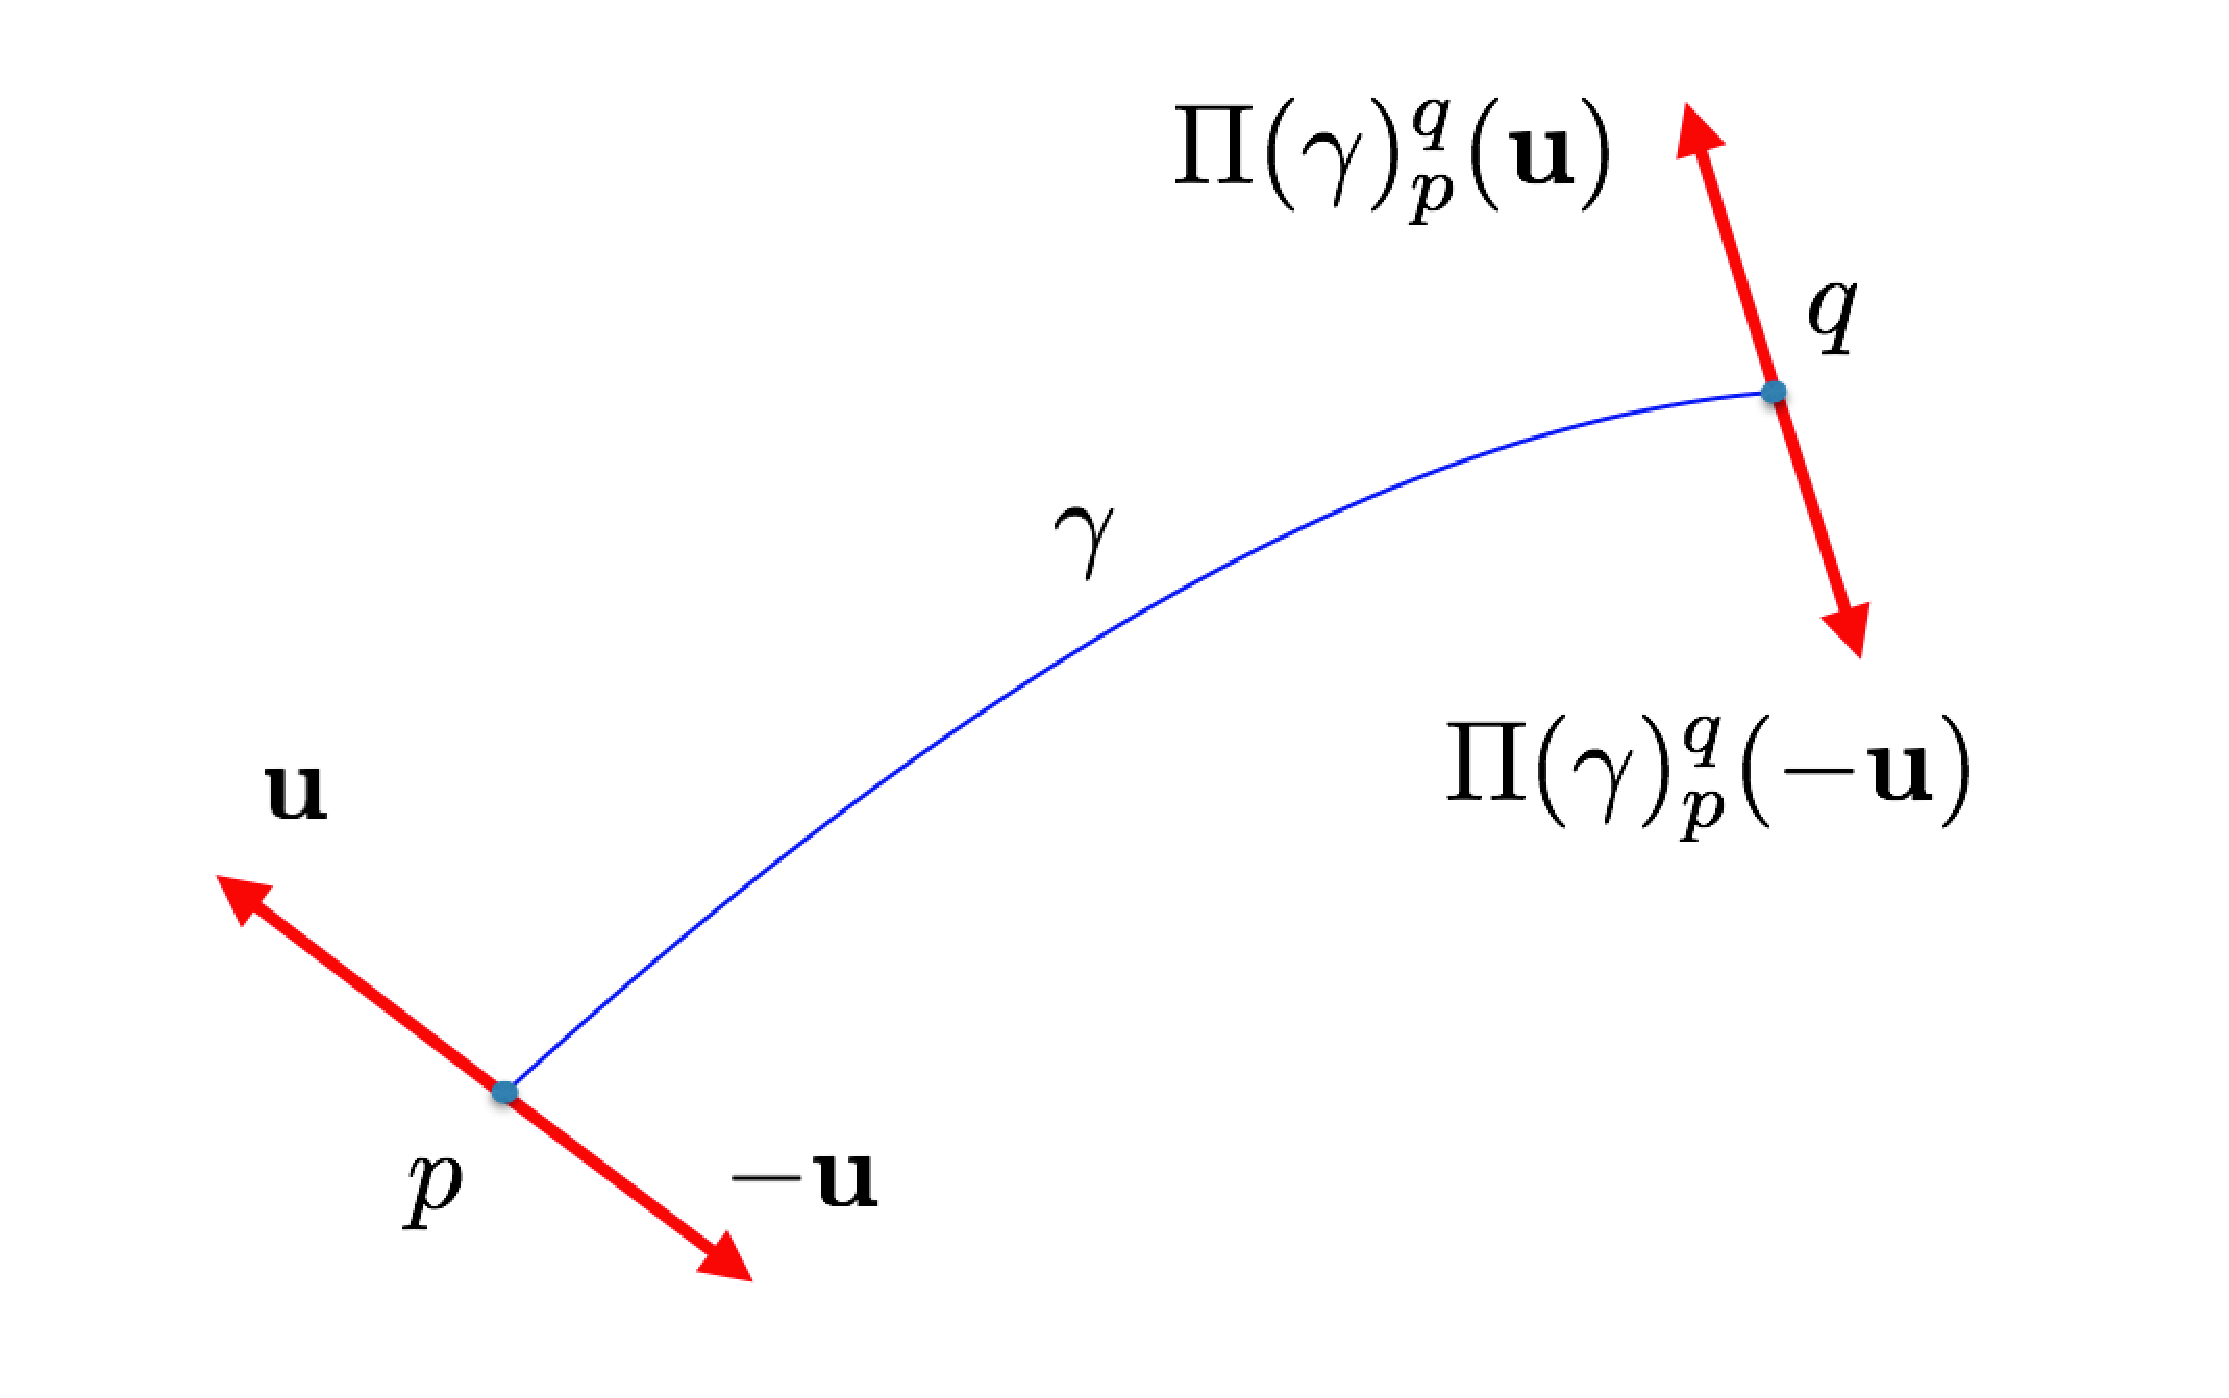
\includegraphics[width=6cm]{figures/inversion_1.pdf}
		\caption{First inversion property.}
		\label{fig:inversion_propr1}
	\end{minipage}
	\ \hspace{9mm} \
	\begin{minipage}[b]{4cm}
		\centering
		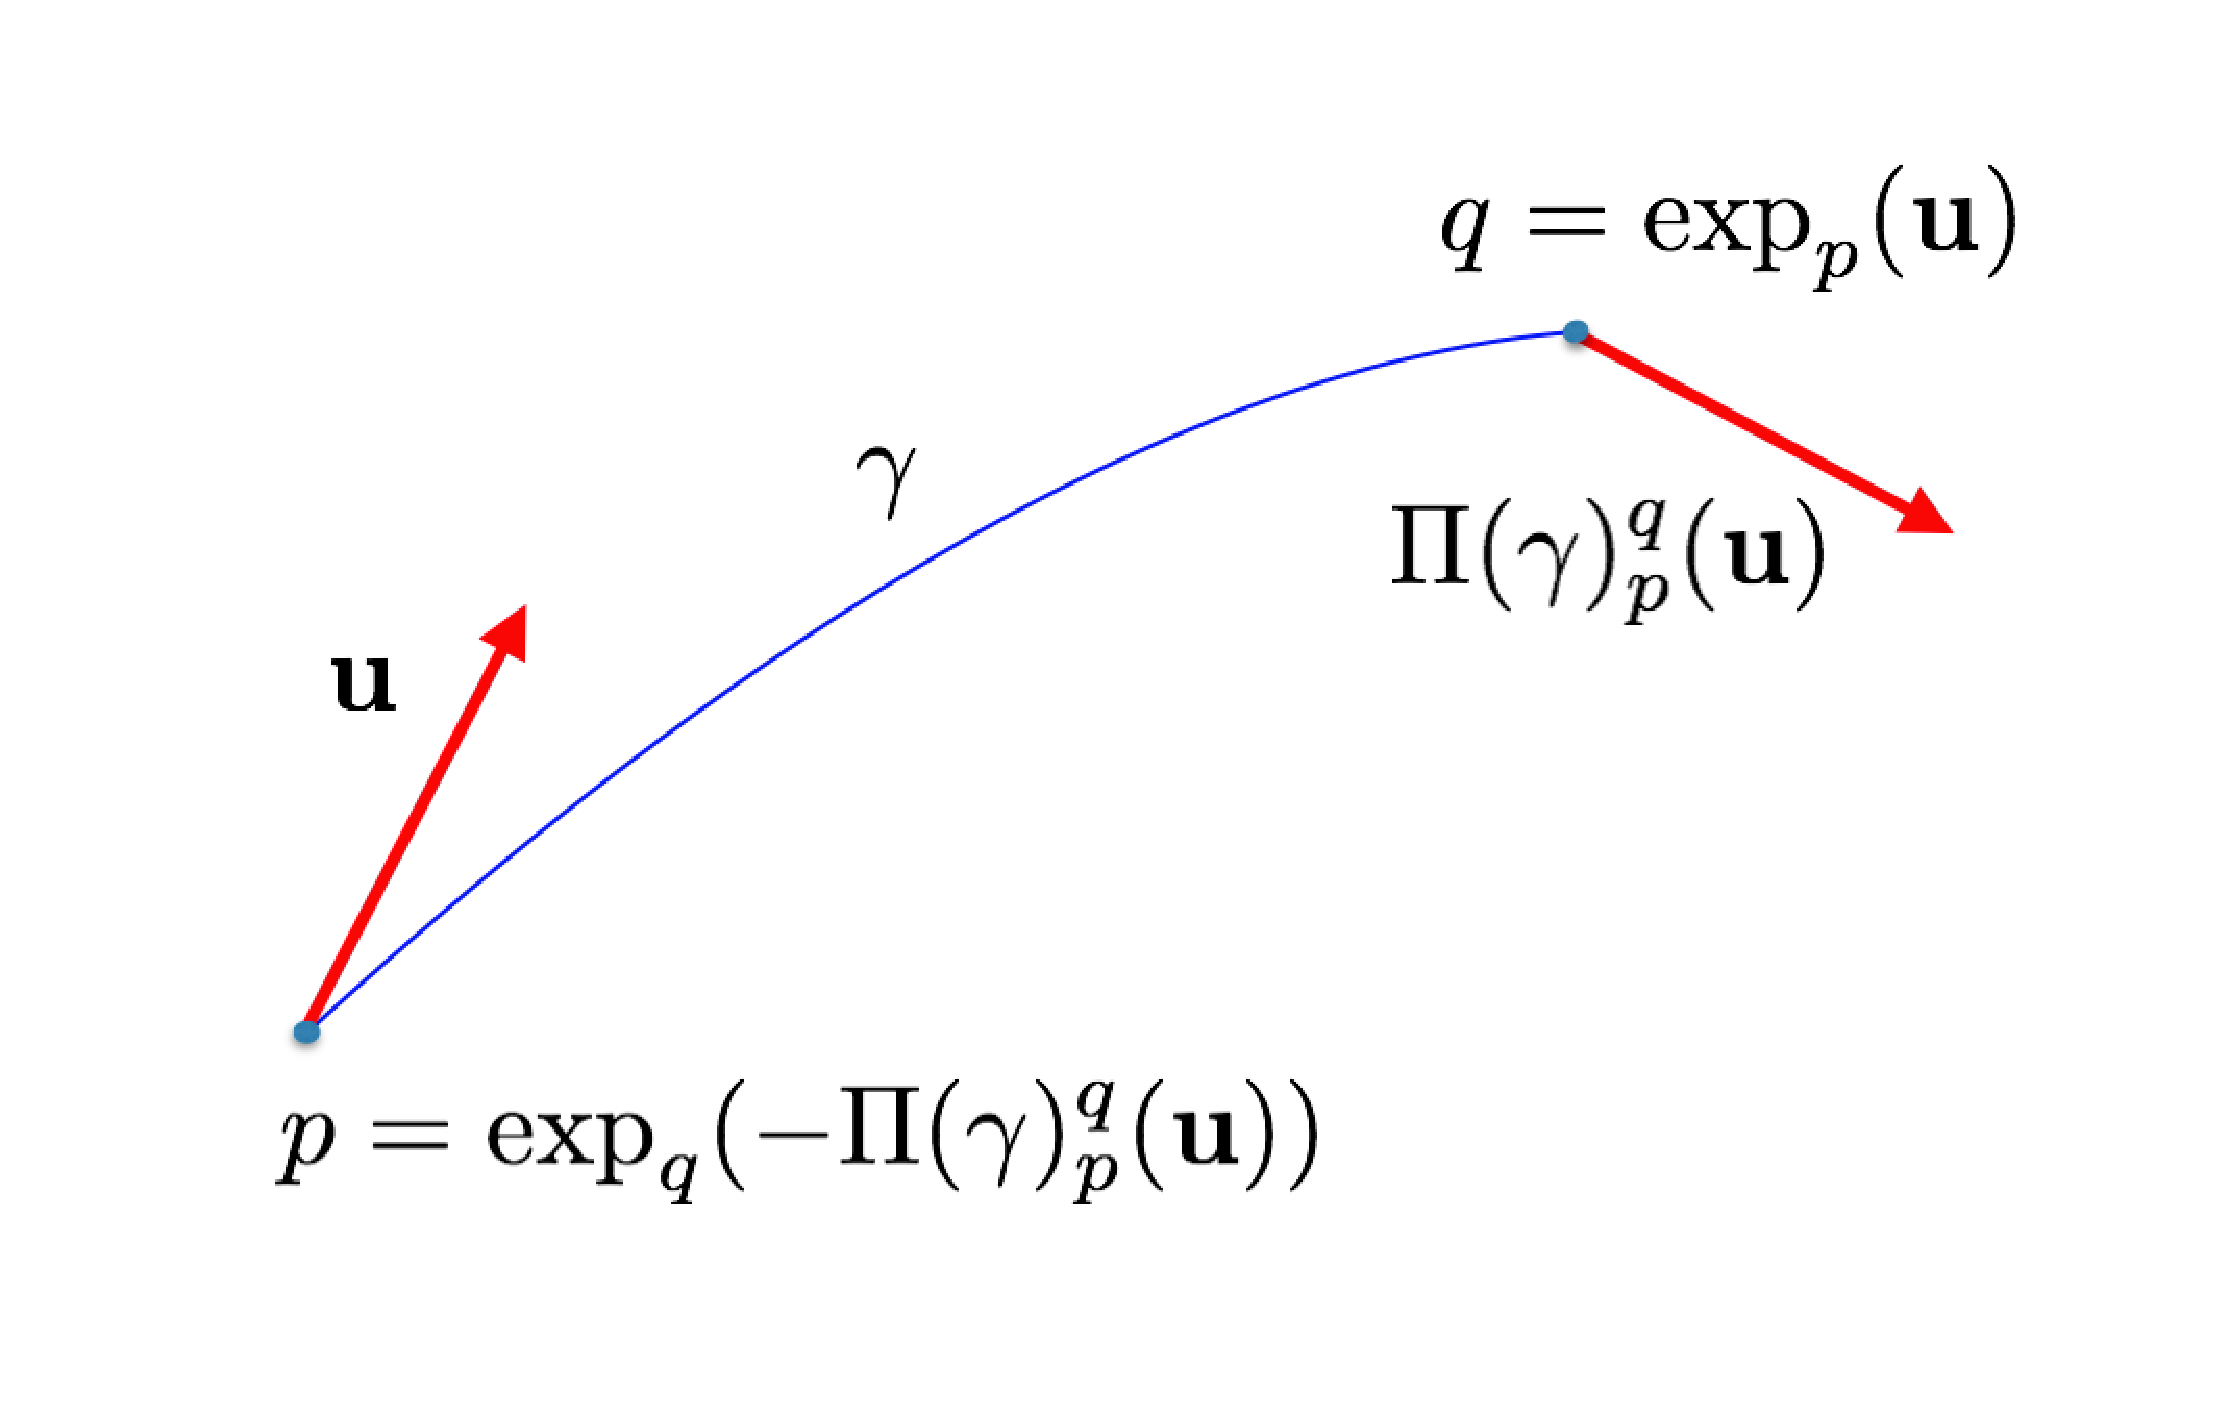
\includegraphics[width=6cm]{figures/inversion_2.pdf}
		\caption{Second inversion property.}
		\label{fig:inversion_propr2}
	\end{minipage}
\end{figure}

\begin{proof}
	The first statement is a consequence of the fact that parallel transport is reversible, conserve the parallelism and it is invariant respect to norm: 
	\begin{enumerate}
		\item[i)] $\Pi(-\gamma)_{q}^{p}\Big(\Pi(\gamma)_{p}^{q}(\mathbf{u})\Big) = \mathbf{u}$ where $-\gamma$ corresponds to $\gamma$ walked in the opposite direction.
		\item[ii)] $\Pi(\gamma)_{p}^{q}(\mathbf{u})$ is parallel in the same tangent space to $\Pi(\gamma)_{p}^{q}(\lambda \mathbf{u})$ for any nonzero $\lambda$.
		\item[iii)] $\euclideanMetric{\Pi(\gamma)_{p}^{q}(\mathbf{u})} = \euclideanMetric{\mathbf{u}}$ 
	\end{enumerate}
	For the second statement, if $q = \exp_{p}(\mathbf{u})$ then it exists a curve $\gamma$ that is a geodesics and connects $p$ with $q$:
	\begin{align*}
		\exp_{p}(\mathbf{u}) = \gamma(1;\mathbf{u}, p) 
		\qquad 
		\nabla_{\dot{\gamma}}\dot{\gamma}=0
		\qquad
		\gamma(0) = p
		\qquad
		\gamma(1) = q
	\end{align*}
	On the other side, if $p = \exp_{q}(-\Pi(\gamma)_{p}^{q}(\mathbf{u}))$, then it exists a curve $\beta$ that is a geodesic and connect $q$ with $p$: 
	\begin{align*}
		\exp_{q}(-\Pi(\gamma)_{p}^{q}(\mathbf{u}))= \beta(1;-\Pi(\gamma)_{p}^{q}(\mathbf{u}), q) 
		\qquad 
		\nabla_{\dot{\gamma}}\dot{\beta}=0
		\qquad
		\beta(0) = q
		\qquad
		\beta(1) = p
	\end{align*}
	Since there is a unique curve that satisfies the condition of being geodesic between two points, we have $\gamma = -\beta$. Therefore, if $q = \exp_{p}(\mathbf{u})$, then
	\begin{align*}
		p &=  \gamma(0;\mathbf{u}, p) = \beta( 1;-\Pi(\gamma)_{p}^{q}(\mathbf{u}), q) 
	\end{align*}
	 which implies $p = \exp_{q}(-\Pi(\gamma)_{p}^{q}(\mathbf{u}))$. On the other side, if $p = \exp_{q}(-\Pi(\gamma)_{p}^{q}(\mathbf{u}))$, then 
	\begin{align*}
	q &= \beta( 0;-\Pi(\gamma)_{p}^{q}(\mathbf{u}), q)  = \gamma(1;\mathbf{u}, p) 
	\end{align*}
	which implies $q = \exp_{p}(\mathbf{u})$.
\end{proof}

\begin{prop}
	Let $\mathbb{G}$ be a finite dimensional connected Lie group defined with a Cartan connection $\nabla$ and $\mathbf{u}$ tangent vector in $ T_{e}\mathbb{G}$. Let $\gamma$ be a geodesic defined on $\mathbb{G}$ such that $\gamma(0) = e$, $\dot{\gamma}(0) =\mathbf{u}$ and $p = \gamma(1)$, point in the Lie group. Let $\beta$ be the curve over $\mathbb{G}$ defined as $\beta(t) = p\circ \gamma(t)$, then the two following conditions hold:
	\begin{enumerate}
		\item If $\nabla$ is a Cartan connection then $\beta$ is a geodesic.
		\item For $\mathbf{u}_{p} := D(L_{p})_{e}(\mathbf{u}) \in T_{p}\mathbb{G}$, push forward of the left-translation:
		\begin{align}\label{eq:lemma_pt}
		\exp_{p}(t\mathbf{u}_{p}) = p\circ \exp_{e}( t D(L_{p^{-1}})_{p}(\mathbf{u}_{p}) ) 
		= p\circ \exp_{e}(t\mathbf{u})
		\end{align}
	\end{enumerate}
\end{prop}
\begin{proof}
	The first statement belongs to the general theory and it is not proved here: geodesics are left-invariant for a Cartan connection (see \cite{do1992riemannian}). To prove the second statement we consider the properties of $\beta$ that directly follows from the definition:
	\begin{align*}
		\beta(0) &= p\circ e = p \\
		\dot{\beta}(0) &= DL_{p}(e)\mathbf{u}\in T_{p}\mathbb{G}
	\end{align*}
	For simplicity $\dot{\beta}(0) $ was indicated with $\mathbf{u}_{p}$. Considering $\beta(1)$ we have: 
	\begin{align*}
		   \beta(1) = p\circ \gamma(1) 
						= p\circ \exp_{e}(\mathbf{u}) 
						= \exp_{p}( DL_p(e) \mathbf{u} ) 
						= \exp_{p}( \mathbf{u}_{p} ) 
	\end{align*}
	where the third equality comes from the change of base formulas for affine exponential \ref{eq:DL_DR}. Following the same deduction and from the linearity of the differential, we have, for any $t\in [ 0,1 ]$:
	\begin{align*}
	\beta(t) = p\circ \gamma(t) 
	= p\circ \exp_{e}(t\mathbf{u}) 
	= \exp_{p}( tDL_p(e) \mathbf{u} ) 
	= \exp_{p}( t\mathbf{u}_{p} ) 
	\end{align*}
\end{proof}

\begin{lemma}
	Let $\mathbb{G}$ be a finite dimensional connected Lie group, $p,q,r$ points of $\mathbb{G}$ belonging to the cut locus. If exists an $\epsilon$ such that 
	\begin{align*}
		\euclideanMetric{\log{(p\circ q)}  - \log{(r)}}< \epsilon
	\end{align*}
	then it follows
	\begin{align*}
	\euclideanMetric{\log{(p)}  - \log{(q^{-1} \circ r)}}< \epsilon
	\end{align*}
\end{lemma}
Intuitively, the lemma states that if $p\circ q \simeq r $ then $p \simeq q^{-1} \circ r $.

The following theorem is an application of the pole ladder \cite{lorenzi2011schild} for the computation of the exponential that will underpin one of the numerical methods for the computation of the log-composition.
\begin{theorem}\label{th:local_approximation_theorem}
	Let $\mathbb{G}$ be a finite dimensional connected Lie group defined with a Cartan connection $\nabla$. 
	Given two vectors $\mathbf{u}, \mathbf{v}$ in the internal cut locus of $\mathfrak{g}$, such that 
	$p = \exp_{e}(\mathbf{u}) $ and	$q = \exp_{e}(\mathbf{v})$, with $\alpha$ integral curve of $\mathbf{u}$,
	\begin{align*}
	\alpha : [0,1] \rightarrow \mathbb{G} \quad \alpha(0) = e  \quad \alpha(1) = p \quad
	\dot{\alpha}(0) = \mathbf{u}
	\end{align*}
	and for $\mathbf{v}_{p}^{\parallel}$ parallel transport of $\mathbf{v}$
	\begin{align*}
	\mathbf{v}_{p}^{\parallel} =  \Pi(\alpha)_{e}^{p}(\mathbf{v})
	\end{align*}
	and $\mathbf{v}_{e}^{\parallel}$ pull-back of the left translation of  the previous vector
	\begin{align*}
	 \mathbf{v}_{e}^{\parallel} := D(L_{p^{-1}})_{e}( \mathbf{v}_{p}^{\parallel})
	\end{align*}
	it follows that:
	\begin{align*}
		\euclideanMetric{
			\log_{e}(\exp_{e}(\mathbf{v}_{e}^{\parallel} ))
			-
			\log_{e}(\exp_{e}\big(\frac{\mathbf{u}}{2}\big)   
				\circ  \exp_{e}(\mathbf{v}) 
				\circ \exp_{e}\big(-\frac{\mathbf{u}}{2}\big))
			} \leq\euclideanMetric{[\mathbf{u}, \mathbf{v}]}
	\end{align*}
\end{theorem}
The statement of this fairly intricate theorem involves a construction that can be visualized in figure \ref{fig:theorem_pict}.
\begin{figure}[htbp]
	\centering
	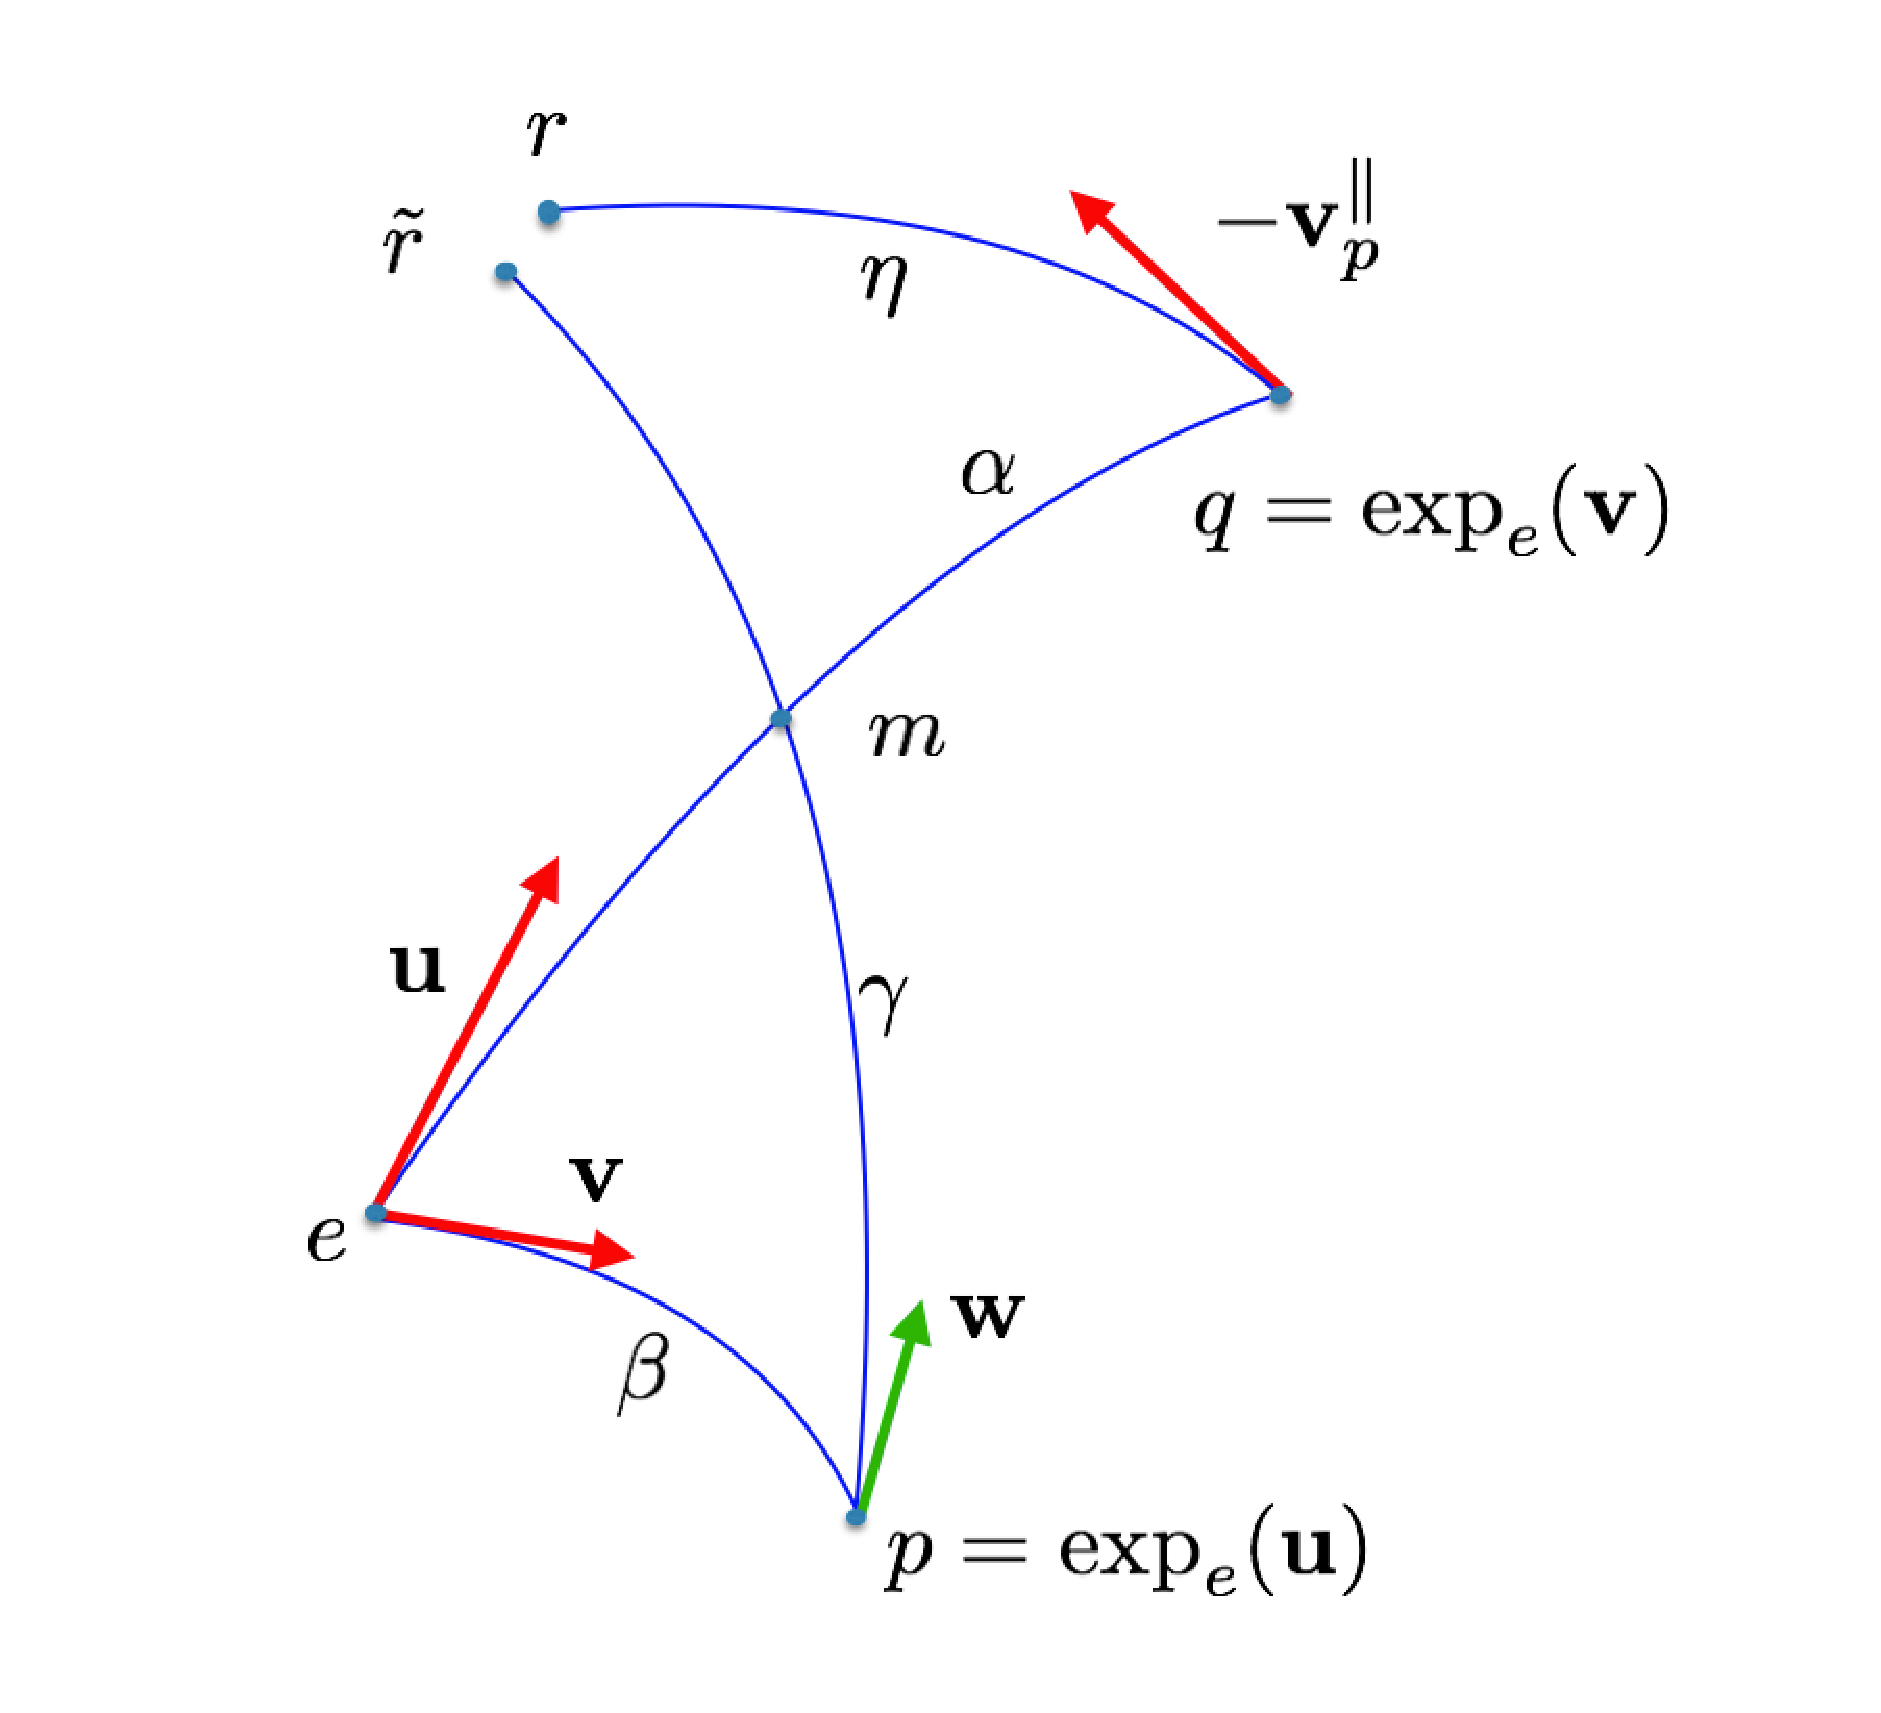
\includegraphics[width=8.5cm]{figures/theorem_pict.pdf}
	\caption{Pole ladder applied to parallel transport.}
	\label{fig:theorem_pict}
\end{figure}
\begin{proof}
	Let $m \in \mathbb{G}$ be the midpoint of the curve $\alpha$, $m = \alpha(1/2) = \exp_{e}(\frac{\mathbf{u}}{2})$ and let $\gamma$ be the geodesic between $q = \exp_{e}(\mathbf{v}) $ and $m$:
	\begin{align*}
	\gamma(0) = q 
	\qquad
	\gamma(1) = m
	\qquad
	\nabla_{\dot{\gamma}} \dot{\gamma} = 0
	\end{align*}
	If $\mathbf{w}$ is the tangent vector of $\gamma$ defined at $q$ such that $\dot{\gamma}(0) = \mathbf{w}$, it follows from the change of base formula \ref{eq:DL_DR} that 
	\begin{align*}
	\gamma(t) = \exp_{q}(t\mathbf{w}) 
	= 
	q \circ \exp_{e}(DL_{p^{-1}}(e)(t\mathbf{w})) 
	= 
	\exp_{e}(\mathbf{v})  \circ \exp_{e}(t DL_{p^{-1}}(e)\mathbf{w}) 
	\end{align*}
	And by construction, we can move from the identity $e$ to $m$ directly walking the geodesic $\alpha$ or passing through $q$. It follows that
	\begin{align*}
		\exp_{q}(\mathbf{w}) &= \exp_{e}(\frac{\mathbf{u}}{2})\\
		q\circ \exp_{e}(DL_{q^{-1}}(e)(\mathbf{w})) &= \exp_{e}(\frac{\mathbf{u}}{2})\\
		\exp_{e}(DL_{q^{-1}}(e)(\mathbf{w})) &= \exp_{e}(-\mathbf{v})\circ\exp_{e}(\frac{\mathbf{u}}{2})
	\end{align*}
	Let $\eta$ be the integral curve of the tangent vector $-\mathbf{v}_{p}^{\parallel}$ at $p$. We define two new points, $r := \eta(1)$ and $\tilde{r} :=\gamma(2)$ where $\gamma$ is the integral curve of $2\mathbf{w}$.\\
	On one side we have:
	\begin{align*}
		\tilde{r} = \gamma(2) &= \exp_q(2\mathbf{w}) = q \circ\exp_{e}(DL_{q^{-1}}(e)(2\mathbf{w})) \\
		&= \exp_{e}(\mathbf{v})\circ\exp_{e}(2DL_{q^{-1}}(e)\mathbf{w}) \\
		&= \exp_{e}(\mathbf{v})\circ\exp_{e}(DL_{q^{-1}}(e)\mathbf{w})^2 \\
		&= \exp_{e}(\mathbf{v})\circ\exp_{e}(\exp_{e}(-\mathbf{v})\circ\exp_{e}(\frac{\mathbf{u}}{2}))^2 \\
		&= \exp_{e}(\frac{\mathbf{u}}{2})\circ \exp_{e}(-\mathbf{v})\circ\exp_{e}(\frac{\mathbf{u}}{2})
	\end{align*}
	On the other side:
	\begin{align*}
		r = \eta(1) &= \exp_{p}(-\mathbf{v}_{p}^{\parallel}) = p \circ\exp_{e}(DL_{p^{-1}}(e)(-\mathbf{v}_{p}^{\parallel})) \\
		&= \exp_{e}(\mathbf{u})\circ\exp_{e}(-DL_{p^{-1}}(e)\mathbf{v}_{p}^{\parallel}) \\
		&= \exp_{e}(\mathbf{u})\circ \exp_{e}(-\mathbf{v}_{e}^{\parallel})
	\end{align*}
	having indicated $DL_{p^{-1}}(e)\mathbf{v}^{\parallel}$ with $\mathbf{v}_{e}^{\parallel}$ for brevity.\\
	By geometrical construction, we have that if the space has no curvature (or equivalently, the Lie group is commutative), $r=\tilde{r}$. Therefore, using the change of signs property \ref{prop:lie_inversion_property}
	\begin{align*}
		\exp_{e}(\mathbf{u})\circ \exp_{e}(-\mathbf{v}_{e}^{\parallel})
		=
		\exp_{e}(\frac{\mathbf{u}}{2})\circ \exp_{e}(-\mathbf{v})\circ\exp_{e}(\frac{\mathbf{u}}{2})
		\\
		\exp_{e}(\mathbf{v}_{e}^{\parallel})
		=
		\exp_{e}(\frac{\mathbf{u}}{2})\circ \exp_{e}(\mathbf{v})\circ\exp_{e}(-\frac{\mathbf{u}}{2})
	\end{align*}
	When the space is curved, again by construction, it follows that
	\begin{align*}
		\euclideanMetric{r-\tilde{r}} \leq \euclideanMetric{[\mathbf{u},\mathbf{v}]}
	\end{align*}
	As a consequence of the previous lemma and observing that if $p$ and $q$ are in the cut locus, than also $r$ and $\tilde{r}$ are in the cut locus, we have finally reach the thesis:
	\begin{align*}
		\euclideanMetric{
			\log_{e}(\exp_{e}(\mathbf{v}_{e}^{\parallel} ))
			-
			\log_{e}(\exp_{e}\big(\frac{\mathbf{u}}{2}\big)   
			\circ  \exp_{e}(\mathbf{v}) 
			\circ \exp_{e}\big(-\frac{\mathbf{u}}{2}\big))
		} 
		\leq
		\euclideanMetric{[\mathbf{u}, \mathbf{v}]}
	\end{align*}
\end{proof} 

The previous result can be reformulated as the approximation:
\begin{align}\label{eq:parallel_transport_main_approximation}
\exp_{e}(\mathbf{v}_{e}^{\parallel}) 
\simeq
\exp_{e}\big(\frac{\mathbf{u}}{2}\big)   
\circ  \exp_{e}(\mathbf{v}) 
\circ \exp_{e}\big(-\frac{\mathbf{u}}{2}\big)
\end{align}
that will turn out to be the main tool for the computation of the log-composition using parallel transport.

In the next section we present the numerical methods for the computation of the log composition.

% % % % % % % % % % % % % % % % % % % % % % % % % % % % % % % % % % % % % %
% % 
% % % % % % % % % % % % % % % % % % % % % % % % % % % % % % % % % % % % % %
\section{Numerical Computations of the Log-composition}

In this section we provide explicit formulas for the computation of the log composition:
\begin{align}\label{eq:main_def_log_composition}
\mathbf{v}_{1}\oplus \mathbf{v}_{2} =  \log(\exp(\mathbf{v}_1)\circ \exp(\mathbf{v}_2))
\end{align}
using the tools introduced in the previous sections.

% % % % % % % % % % % % % % % % % % % % % % % % % % % % % % % % % % % % % %
% % 
% % % % % % % % % % % % % % % % % % % % % % % % % % % % % % % % % % % % % % 
\subsection{Truncated BCH formula for the Log-composition}\label{se:bch_formula}

As said in the end of section \ref{se:lie_exp_log_comp_bch} the Lie log-composition posses a closed form, the BCH formula, defined as the solution of the equation $\exp(\mathbf{w}) = \exp(\mathbf{u}) \circ \exp(\mathbf{v})$, for $\bf{u}$ and $\bf{v}$ \emph{analytic} elements in the Lie algebra $\mathfrak{g}$:
\begin{align}\label{eq:bch_definition}
	BCH(\mathbf{u},\mathbf{v}) 
	= 
	\mathbf{u} + \mathbf{v} + \frac{1}{2}[\mathbf{u},\mathbf{v}] + \frac{1}{12}([\mathbf{u},[\mathbf{u},\mathbf{v}]]
	+ [\mathbf{v},[\mathbf{v},\mathbf{u}]]) - \frac{1}{24}[\mathbf{v},[\mathbf{u},[\mathbf{u},\mathbf{v}]]] +... 
\end{align}
It consists of an infinite series of Lie bracket whose asymptotic behaviour cannot be predicted only from the coefficient of each nested Lie bracket term. In practical applications it can be computed using its \emph{approximation of degree} $k$, defined as the sum of the BCH terms having no more than $k$ nested Lie bracket. This convention is also coherent with the degree of the BCH expressed as polynomial formal series of adjoint operators (see next section \ref{se:taylor_expansion}):
\begin{align*}
BCH^{0}(\mathbf{u},\mathbf{v}) &= \mathbf{u} + \mathbf{v} \\
BCH^{1}(\mathbf{u},\mathbf{v}) &=  \mathbf{u} + \mathbf{v} + \frac{1}{2}[\mathbf{u},\mathbf{v}] \\
BCH^{2}(\mathbf{u},\mathbf{v}) &=  \mathbf{u} + \mathbf{v} + \frac{1}{2}[\mathbf{u},\mathbf{v}] + \frac{1}{12}([\mathbf{u},[\mathbf{u},\mathbf{v}]] + [\mathbf{v},[\mathbf{v},\mathbf{u}]]) \\
BCH^{3}(\mathbf{u},\mathbf{v}) &=  \mathbf{u} + \mathbf{v} + \frac{1}{2}[\mathbf{u},\mathbf{v}] + \frac{1}{12}([\mathbf{u},[\mathbf{u},\mathbf{v}]] + [\mathbf{v},[\mathbf{v},\mathbf{u}]])- \frac{1}{24}[\mathbf{v},[\mathbf{u},[\mathbf{u},\mathbf{v}]]] 
\end{align*}
In numerical computations nested Lie brackets can raise several issue, in particular when $\mathbf{u}$ and $\mathbf{v}$ are not close to the origin. Assuming that, as often happens for practical applications in imaging registration $\mathbf{v}$ is smaller than $\mathbf{u}$, we define a intermediate degree for the truncated BCH formula, between $1$ and $2$:
\begin{align*}
BCH^{3/2}(\mathbf{u},\mathbf{v}) &=  \mathbf{u} + \mathbf{v} + \frac{1}{2}[\mathbf{u},\mathbf{v}] + \frac{1}{12}[\mathbf{u},[\mathbf{u},\mathbf{v}]]
\end{align*}

Truncated BCH formulas can be considered as a first step toward the numerical approximations of the log-composition $\mathbf{u}\oplus \mathbf{v}$. They still have some limitations as the fact that they do not provide any information about the error carried by each term, and they work under the assumption that $\mathbf{u}$ and $\mathbf{v}$ are analytic, so when we can expressed locally with a convergent power series, as in the case of tangent vectors to matrix Lie group. Additional limitation can be found when applied to stationary velocity fields. This will be one of the topic of section \ref{se:log_composition_SVF}.


% % % % % % % % % % % % % % % % % % % % % % % % % % % % % % % % % % % % % %
% % 
% % % % % % % % % % % % % % % % % % % % % % % % % % % % % % % % % % % % % % 
\subsection{Taylor Expansion Method for the Log-composition}\label{se:taylor_expansion}

A more sophisticated numerical method to manage the nested Lie brackets for the computation of the log-composition is based on the Taylor expansion. \\
As shown in the appendix of \cite{klarsfeld1989baker} the terms of the BCH can be recollected using the Hausdorff method: each of the therms containing the n-th power of the vector $\mathbf{v}$ are collected together in the formal series $A^{n}$. Therefore
\begin{align*}
%\mathbf{u}\oplus \mathbf{v}  
BCH(\mathbf{u},\mathbf{v}) 
= 
\mathbf{u} + A^{1} \mathbf{v} + A^{2} \mathbf{v} + A^{3} \mathbf{v} + \cdots
\end{align*}
Given the adjoint map:
\begin{align*}
ad_{\mathbf{u}} : \mathfrak{g}  & \longrightarrow \mathfrak{g}  
\\
\mathbf{v} &\longmapsto ad_{\mathbf{u}}   \mathbf{v} :=  [\mathbf{u}, \mathbf{v}]
\end{align*}
and the multiple adjoint maps, defined as:
\begin{align*}
\text{ad}_{\mathbf{u}}^{n} \mathbf{v} 
&:= [  \underbrace{   \mathbf{u},[\mathbf{u},... [\mathbf{u}}_{\text{n-times}},\mathbf{v}]...]] 
\\
\\
\text{ad}_{\mathbf{u}}^{-n} \mathbf{v} 
&:= [[...[  \mathbf{v}, \underbrace{   \mathbf{u}]...],\mathbf{u}}_{\text{n-times}}]
= (-1)^n \text{ad}_{\mathbf{u}}^{n} \mathbf{v} 
\end{align*}
it can be demonstrated that then the operator $A^{1}$, when applied to $\mathbf{v}$ provides the linear part of $\mathbf{v}$ in the BCH formula and can be written as:
\begin{align*}
A^{1}
= 
\frac{  
	\text{ad}_{\mathbf{u}}^{-1} 
	}{
	\exp{(\text{ad}_{\mathbf{u}})}-1
	}
=
\sum_{n=0}^{\infty} \frac{(-1)^nB_{n}}{n!} \text{ad}_{\mathbf{u}}^{ - n} 
=
\sum_{n=0}^{\infty} \frac{B_{n}}{n!} \text{ad}_{\mathbf{u}}^{ n} 
\end{align*}
where $\lbrace B_{n} \rbrace_{n=0}^{\infty} $ is the sequence of the second-kind Bernoulli number. If first-kind Bernoulli number are used, then each term of the summation must be multiplied for $(-1)^{n}$, as did for example in \cite{klarsfeld1989baker}. The denominator is defined within the structure of the formal power series ring \cite{mariconda2013calcolo}.\\
In conclusion, the log-composition can expressed as:
\begin{align*}
\mathbf{u}\oplus \mathbf{v}  
&= 
\mathbf{u} + 
\frac{  
	\text{ad}_{\mathbf{u}}^{-1} 
}{
\exp{(\text{ad}_{\mathbf{u}})}-1
} \mathbf{v}  
+ 
\mathcal{O}(\mathbf{v} ^2) 
\end{align*}
\begin{align}\label{eq:taylor}
\mathbf{u}\oplus \mathbf{v}  
&=
\mathbf{u} 
+
\sum_{n=0}^{\infty} \frac{B_{n}}{n!} \text{ad}_{\mathbf{u}}^{ n} 
\mathbf{v}  
+
\mathcal{O}(\mathbf{v} ^2)
\end{align}
that will turn out to be an important tool for the computation of the log-composition in the finite dimensional case. 

% % % % % % % % % % % % % % % % % % % % % % % % % % % % % % % % % % % % % %
% % 
% % % % % % % % % % % % % % % % % % % % % % % % % % % % % % % % % % % % % % 
\subsection{Parallel Transport Method for the Log-composition}
To obtain a numerical computation for the log-composition using parallel transport, we have to consider two assumptions: 
\begin{enumerate}
	\item If $\mathbf{v}_{e}^{\parallel} $ is defined as in theorem \ref{th:local_approximation_theorem}, then
	\begin{align*}
	\euclideanMetric{
		\mathbf{u}\oplus \mathbf{v}  
		-
		(
		\mathbf{u} + \mathbf{v}_{e}^{\parallel} 
		)
	} 
	\leq 
	\euclideanMetric{
		[\mathbf{u}, \mathbf{v}]
		}
	\end{align*}
	\item If the vector $\mathbf{u}\in\mathfrak{g}$ is small enough, then:
		\begin{align*}
		\exp(\mathbf{u}) \simeq e + \mathbf{u}
		\end{align*}
\end{enumerate}
The first assumption is a consequence of geometrical intuition. On a flat space, or a space with no curvature, the geodesics are straight lines, and $\mathbf{u}\oplus \mathbf{v} = \mathbf{u} + \mathbf{v} $ that is equal, again intuitively, to the sum of $\mathbf{u}$ with the parallel transported of $\mathbf{v}$ to the point $\exp_{e}(\mathbf{u})$, indicated with $\mathbf{v}_{p}^{\parallel} $ (see figure \ref{fig:u_plus_v_parallel_transported}). It is not possible to sum two vectors belonging to two different planes, therefore we have to consider the transported $\mathbf{v}_{e}^{\parallel} $ instead of $\mathbf{v}_{p}^{\parallel} $. In addition, when the space is not flat, the equalities $\mathbf{u}\oplus \mathbf{v} = \mathbf{u} + \mathbf{v} $ do not holds.

% u_plus_v_parallel_transported
\begin{figure}[htbp]
	\centering
	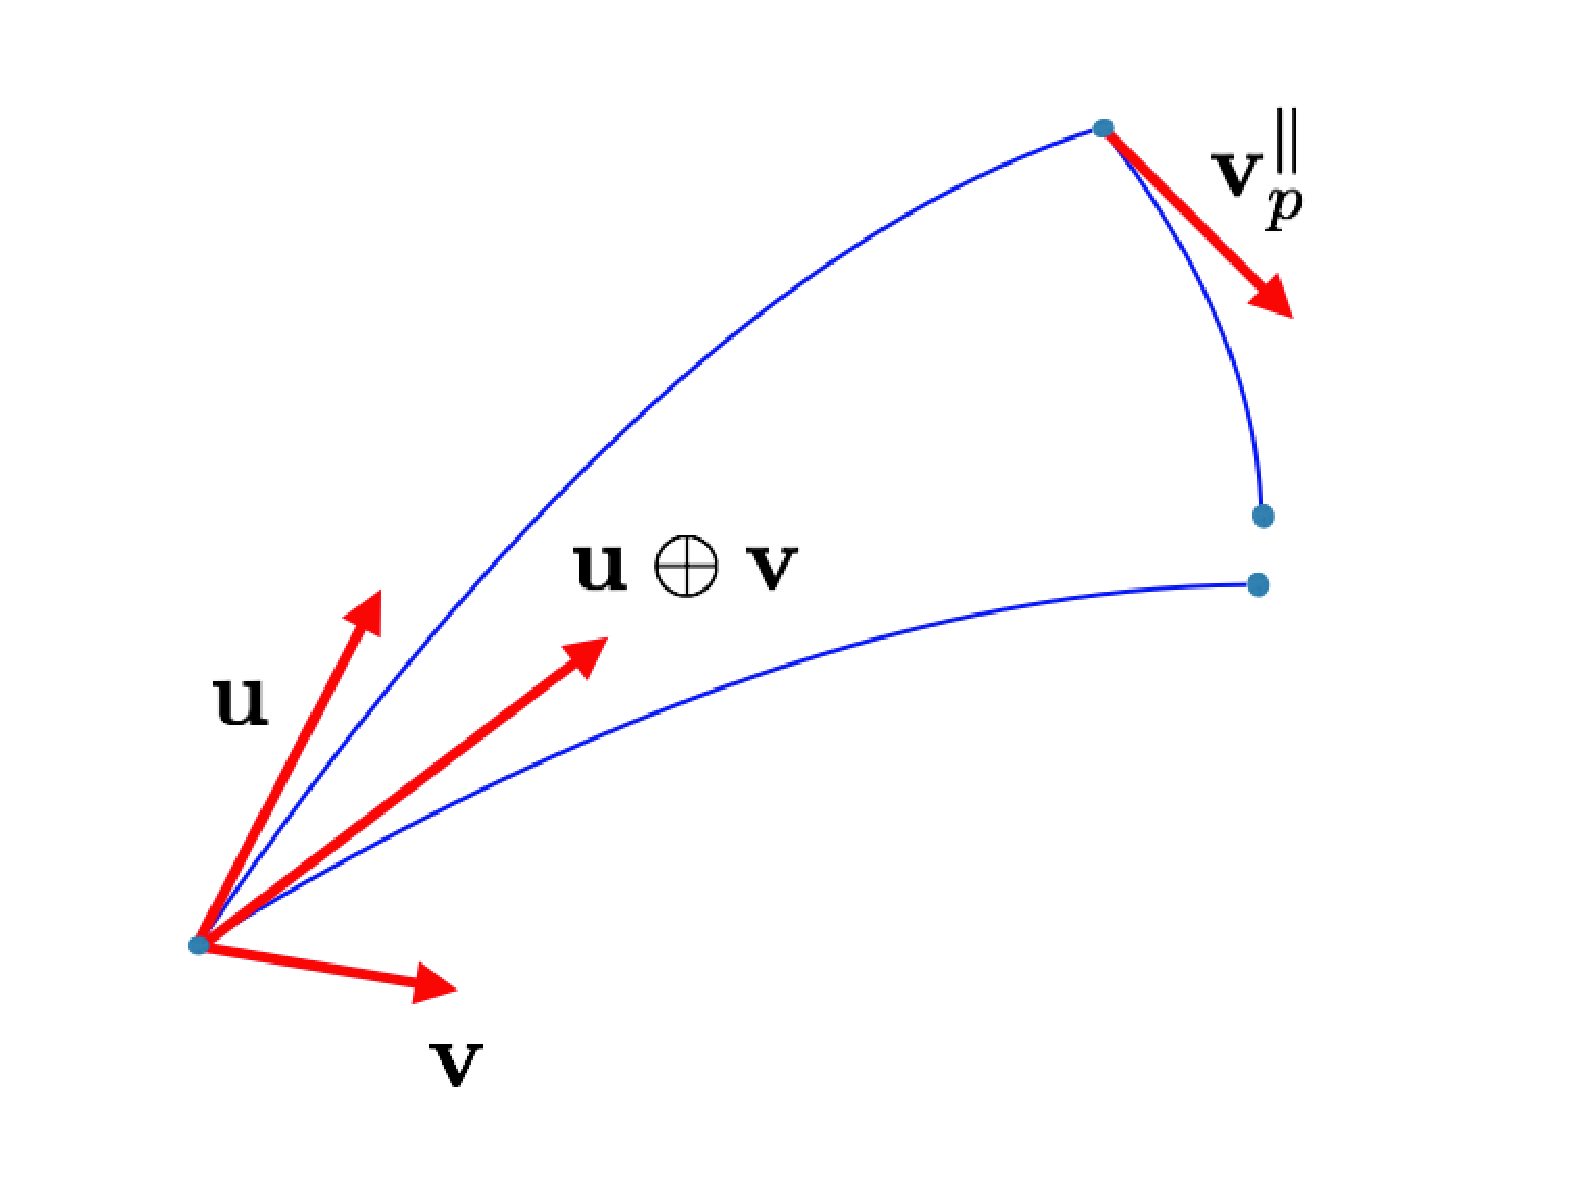
\includegraphics[width=6.5cm]{figures/u_plus_v_parallel_transported.pdf}
	\caption{Representation of the intuitive idea of the computation of the log-composition using parallel transport.}
	\label{fig:u_plus_v_parallel_transported}
\end{figure}
The validity of the second assumption must be investigated case by case. For example when $\mathbb{G}$ is a matrix Lie group, the formula \ref{eq:exp_as_inf_sum} provides $\exp(\mathbf{u}) = I + \mathbf{u} + \mathcal{O}(\mathbf{u}^2)$. In the case of stationary velocity field, we have that the condition hold when $\mathbf{u}$ is small enough (see proposition 8.6 pag. 163 \cite{younes2010shapes}). More on this will be presented in \ref{se:log_composition_SVF}.

Assuming the validity of these assumptions and from equation \ref{eq:parallel_transport_main_approximation} it follows that 
\begin{align*}
\mathbf{u}\oplus \mathbf{v}
&\simeq
\mathbf{u} + \mathbf{v}_{e}^{\parallel}
\\
e + \mathbf{v}_{e}^{\parallel}
&\simeq
\exp_{e}\big(\frac{\mathbf{u}}{2}\big)   
\circ  \exp_{e}(\mathbf{v}) 
\circ \exp_{e}\big(-\frac{\mathbf{u}}{2}\big)
\end{align*}
Therefore
\begin{align}\label{eq:parallel_transport}
\mathbf{u}\oplus \mathbf{v}
&\simeq
\mathbf{u} 
+
\exp_{e}\big(\frac{\mathbf{u}}{2}\big)   
\circ  \exp_{e}(\mathbf{v}) 
\circ \exp_{e}\big(-\frac{\mathbf{u}}{2}\big)
 -
 e
\end{align}
When working in the infinite dimensional case, the approximation \ref{eq:parallel_transport} holds under the following additional assumption:
\begin{enumerate}
\item[3.] Theorem \ref{th:local_approximation_theorem} holds when the Lie group is infinite dimensional.
\end{enumerate}
An eventual confirmation is at the moment not known to the author. We assume it is true in coherence with what has been said in the introduction, section \ref{se:diffe_util_and_liab} about a naive approach to the infinite dimensional Lie Group theory.

With the truncated BCH and the Taylor expansion, equation \ref{eq:parallel_transport} is the third numerical method for the computation of the log-composition explored in this thesis. The next chapter is devote to introduce two group of transformation - the rigid body transformation and the diffeomorphisms - and to apply the numerical methods presented in this chapter to these cases.




